\section{Introduction}
\label{sec:intro}

High-dimensional embeddings are now first-class data objects in retrieval-augmented generation, recommendation, and real-time observability workloads~\cite{lewis2020rag}. In these settings, vector similarity joins are no longer occasional offline operators; they run continuously over high-rate streams and must satisfy sliding-window semantics under strict latency constraints, in the spirit of modern unbounded stream processing models~\cite{akidau2015dataflow}. This requirement fundamentally changes the systems problem relative to static ANN search~\cite{jegou2011product,malkov2018efficient}: the engine must jointly handle continuous ingestion, timely expiration, and parallel query/verification on shared-memory multicore hardware.

\begin{figure}[t]
	\centering
	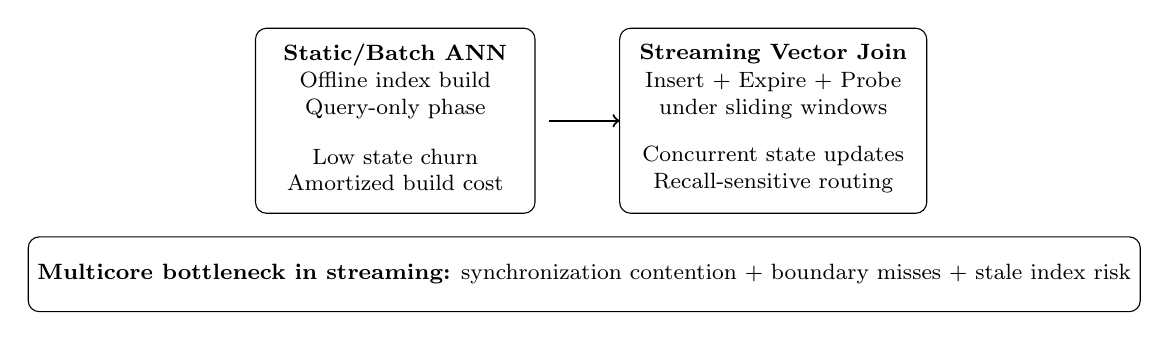
\begin{tikzpicture}[font=\footnotesize, node distance=0.2cm]
		% Left panel: static/batch ANN
		\node[draw, rounded corners, minimum width=3.55cm, minimum height=2.35cm, align=center] (leftbox) at (0,0) {};
		\node[anchor=north] at ([yshift=-0.08cm]leftbox.north) {\textbf{Static/Batch ANN}};
		\node[align=center] at ([yshift=0.32cm]leftbox.center) {Offline index build\\Query-only phase};
		\node[align=center] at ([yshift=-0.62cm]leftbox.center) {Low state churn\\Amortized build cost};

		% Right panel: streaming join
		\node[draw, rounded corners, minimum width=3.9cm, minimum height=2.35cm, align=center] (rightbox) at (4.8,0) {};
		\node[anchor=north] at ([yshift=-0.08cm]rightbox.north) {\textbf{Streaming Vector Join}};
		\node[align=center] at ([yshift=0.32cm]rightbox.center) {Insert + Expire + Probe\\under sliding windows};
		\node[align=center] at ([yshift=-0.62cm]rightbox.center) {Concurrent state updates\\Recall-sensitive routing};

		% Arrow between panels
		\draw[->, thick] (1.95,0) -- (2.85,0);

		% Bottom bottlenecks
		\node[draw, rounded corners, minimum width=8.15cm, minimum height=0.95cm, align=center] at (2.4,-1.95)
		{\textbf{Multicore bottleneck in streaming:} synchronization contention + boundary misses + stale index risk};
	\end{tikzpicture}
	\caption{Motivation: unlike static ANN pipelines, streaming vector joins must maintain correctness and latency under simultaneous ingestion, expiration, and probing.}
	\label{fig:intro-motivation}
\end{figure}

\system addresses this setting with a strategy-driven join architecture that composes four dimensions---join algorithm, partition strategy, window-state type, and index strategy---within a unified runtime. This design enables apples-to-apples comparison of multiple baselines and system choices in one framework, including BruteForce, IVF, HNSW, HDR-Tree, LSH, ClusteredJoin, S3J-style methods, and our VSJoin-oriented path. As illustrated in Figure~\ref{fig:intro-motivation}, a key practical insight is that throughput alone is insufficient: correctness and recall are highly sensitive to partition/state compatibility and runtime routing behavior, especially at high parallelism.

Our VSJoin-oriented path combines partition-local write-friendly indexes with a global read-oriented index layer, plus boundary-aware multicast routing to reduce cross-partition miss probability near decision borders. In the latest implementation, routing uses LSH-based logical partitioning with virtual nodes, where each record is mapped by a stable identity hash and then resolved through an RCU-style assignment table to physical workers. The runtime continuously samples per-subtask load and applies threshold-triggered, bounded remapping using interval load deltas (with smoothed latency/backlog signals), which improves skew robustness without blocking the foreground path. During execution, candidate generation is separated from final verification: indexes provide fast candidate retrieval, while window and similarity checks enforce output correctness under temporal constraints. This separation gives a clean place to trade recall and latency, and it allows us to retain a common verification path across algorithms while varying indexing and partitioning policies.

Implementation-driven evaluation in \system shows two robust execution regimes in current end-to-end testing: (1) a shared-state/shared-index path centered on RoundRobin routing for classic baselines, and (2) a centroid-partitioned path for ClusteredJoin with explicit partition-count and multicast controls. The VSJoin path is integrated into the same runtime with dedicated routing and rebuild mechanisms, and our results show competitive throughput--latency behavior with strong quality in validated workloads. At the same time, we make implementation constraints explicit so that claims remain reproducible under the tested configuration space.

In summary, this paper makes the following contributions:
\begin{itemize}
	\item We present a unified multicore streaming vector-join architecture that exposes algorithm, partition, state, and index policies as first-class strategy knobs.
	\item We design a VSJoin-oriented execution path that combines local/global indexing, LSH-based logical partitioning with virtual nodes, and bounded online remapping for sliding-window workloads.
	\item We provide an implementation-grounded evaluation in \system for end-to-end comparison across multiple baselines under shared infrastructure.
	\item We distill practical compatibility and deployment guidelines for maintaining recall and latency stability at high parallelism.
\end{itemize}

The rest of this paper is organized as follows. Section~\ref{sec:problem-statement} formalizes the problem and motivation. Section~3 presents the core join architecture and method-specific execution paths. Section~\ref{sec:implementation-methodology} describes implementation details and experimental methodology. Section~\ref{sec:results} reports experimental results. Section~\ref{sec:related-work} discusses related work, and Section~\ref{sec:conclusion} concludes.
% \section{Introduction}
% \label{sec:intro}
% \dscf (\dsc) is one of the most important data stream mining operations. 
% In the last decades, \dsc has been widely applied in various real-world scenarios, including network intrusion detection~\cite{KDD99}, social network analysis~\cite{EDMStream:17} and weather forecast~\cite{weather_forecast:2020}. 
% \dsc aims at grouping input tuples according to their attribute similarities on the fly. 
% \modify{In contrast to batch clustering algorithms such as \kmeans~\cite{KMeans:1967,KMeans:1982} or \dbscan~\cite{DBSCAN:1996}, \dsc algorithms are required to handle some data stream characteristics, such as \emph{high data arrival rate} and \emph{occurrence of concept evolution}~\cite{Stream_Clustering_Survey01,Empirical:2018}.}
% % \tony{frequent cluster evolving}, high processing efficiency and low memory footprint
% The processing efficiency and accuracy are both critical concerns of \dsc algorithms~\cite{EmpiricalR:2017,Empirical:2018,DSC_Survey:02}.

% % In the last decades, 
% % numerous \dsc algorithms have been propose. 
% The complex use case scenarios and varying performance metrics motivate the rapid development of numerous \dsc algorithms~\cite{concept_evolution:2010,Clustream:03,Concept_Evolution:11,Concept_Evolution:16}.
% % a large number of \dsc algorithms. 
% % from a number of research communities.
% Despite its prosperity, it is still difficult for researchers and practitioners to determine a suitable \dsc algorithm on real-world workloads with varying characteristics. 
% In particular, there are several fundamental design choices that have different trade-offs and performance behaviours among \dsc algorithms. These design decisions are also highly dependent on each other. Thus, it is non-trivial to discern which ones are better than others and why. 

% % Until now, there has not been a comprehensive evaluation of design choices of \dsc in the literature.
% % p?
% Some prior works~\cite{EmpiricalR:2017,Empirical:2018} have conducted evaluations of \dsc algorithms, but they suffer from several drawbacks:
% (1) \emph{coarse-grained comparison among \dsc algorithms.} 
% Existing studies are limited to giving a coarse-grained analysis of absolute performance among \dsc algorithms. They fail to investigate the design similarities and differences in algorithm design aspects and pinpoint those attributed to the performance differences. 
% % Moreover, prior studies conduct evaluations on a biased narrow subset of \dsc algorithms. 
% (2) \emph{the benchmark settings are problematic.} 
% Previous benchmark settings only contain accuracy metrics while ignoring processing efficiency metrics, which are at least equally crucial. Besides, the used workloads are not able to cover some key characteristics of real-world scenarios, such as the frequency of concept evolution. 
% % (3) \emph{implementations from different codebases.} 
% % Existing studies 
% % % are based on 
% % % of DSC algorithms 
% % lead to misguided experimental results that may be caused by various programming languages, compilers and implementation tricks. 
% % Thus, prior works are not able to fairly reflect and reason the behaviour of \dsc algorithms on complex real-world data with varying characteristics.        
% % \begin{myenumerate}
% %     \item \emph{The benchmark settings are problematic.}
% %         Previous benchmark settings only contain accuracy metrics while ignoring processing efficiency metrics, which are at least equally crucial for \dsc. Besides, the used workloads are not able to cover some key characteristics of real-world scenarios, such as the frequency of concept evolution. Moreover, they are based on implementations of \dsc algorithms from different codebases, leading to misguided experimental results that may be caused by various programming languages, compilers and implementation tricks.
% %         Therefore, the existing works are not sufficient to fairly reflect the behaviour of \dsc algorithms on complex real-world data with varying characteristics.
% %     \item \emph{Only coarse-grained comparison among \dsc algorithms.} 
% %         To the best of our knowledge, existing studies are limited to giving a coarse-grained analysis of absolute performance among \dsc algorithms. They fail to investigate the design similarities and differences in algorithm design aspects and pinpoint those attributed to the performance differences. 
% %         Moreover, these studies conduct evaluations on a biased narrow subset of \dsc algorithms. 
% %         % without fully explaining why selecting them. 
% % \end{myenumerate}

% % but these studies are limited to giving a coarse-grained analysis of absolute performance among \dsc algorithms. They fail to investigate the design similarities and differences in algorithm design aspects and pinpointing those attributing to the performance differences.
% % The community needs 
% % 1) \emph{a comprehensive evaluation based on a benchmark involving varying workload characteristics concerning both clustering accuracy and processing efficiency.}
% % and
% % 2) \emph{a fine-grained analysis for \dsc algorithms by decoupling algorithms into common design aspects.
% % % based on design aspects commonly built among them.
% % } 

% In this paper, we perform an in-depth study of key design aspects of \dsc algorithms: 
% (1) window model, (2) outlier detection mechanism, (3) summarizing data structure, and (4) offline refinement strategy. For each design aspect, there are multiple design options that lead to different \dsc algorithms that behave differently under varying workloads. 
% As part of this investigation, 
% we made a good faith effort to implement all of these approaches in the same framework, called \textbf{\system} from scratch using C++. We open-source \system at \url{https://anonymous.4open.science/r/Sesame-B728}. \system follows a modular design, which clearly separates key design aspects. This eliminates the differences among existing implementations caused by programming languages and compilers.  % Ultimately, existing stream clustering algorithms can be constructed by composing software components implemented for each design aspect. 
% % This allows us to better comprehend the different trade-offs and performance behaviours among algorithms in a much finer granularity.


% % k?
% Based on \system, we conduct our study using four real-world and two synthetic workloads with varying characteristics. Through extensive evaluation, we are able to make a number of novel findings, \modify{such as} 
% (a) each design has its own strength and limitation and none can achieve the highest accuracy and efficiency at the same time;
% (b) \modify{consequently, none of the existing \dsc algorithms can always achieve good performance under varying workload characteristics;}
% % none can always perform the best under different workloads
% and (c) the best choice of each design aspect of \dsc algorithms depends on a number of factors including workload characteristics, optimization targets, as well as the choices made in other design aspects.
% Our findings even promote a novel \dsc algorithm called \emph{Benne}, that combines flexible design choices from four design aspects. It can achieve either the best accuracy or the best efficiency compared to the state-of-the-art on all workloads. 

% % We evaluate based on both the accuracy metrics (i.e., CMM~\cite{CMM:2011} and Purity~\cite{purity:12}) and the performance metrics (i.e., throughput and latency). These metrics are with divergent purposes for evaluating the algorithm's behavior comprehensively. 

% The remaining of this paper is organized as follows: 
% Section~\ref{sec:background} provides an overview of \dsc algorithms and the design of our testbed -- \system.  
% In Sections~\ref{sec:summarizing_data_structure}$\sim$\ref{sec:offline_refinement_strategy}, we discuss the implementation issues and performance trade-offs of various design decisions of \dsc algorithms. We then perform a comprehensive evaluation of them in Section~\ref{sec:evaluation}. 
% Section~\ref{sec:relatedwork} discusses related work, and Section~\ref{sec:conclusion} concludes this study.
% We note that we focus on single-thread execution in this paper, and leave the study of parallelization of \dsc algorithms in future work.
% % Despite their significant differences, they are commonly built around four key design aspects including window model, outlier detection mechanism, summarizing data structure and offline refinement strategy. In each design aspect, there are multiple design options that lead to many existing \dsc algorithms that behave differently under varying workloads. 
% % Various design options in each design aspects lead existing \dsc algorithms to perform significant differently
% % Apart from this, many open-source projects also created their frameworks or libraries involving implementations for some of the \dsc algorithms~\cite{MOA_Web,SAMOA:15}.
% % we notice that a fundamental problem has not yet been answered, which is \emph{``how do these algorithms perform in real-world workloads?''}
% % Despite the recent advance of the CardEst methods, we notice that a fundamental problem has not yet been answered, whichis“to whatextent canthese advanced CardEst methods improve the performance of query optimizers in real-world settings?” Although existing studies have conducted extensive experiments, they suffer from the following shortcomings:
% % 1. \emph{The benchmark settings used for evaluation may not well represent the real-world scenarios.}
% %         Previous benchmark settings only contain accuracy metrics while ignoring processing efficiency metrics, which are at least equally important. Besides, the applied workloads can not cover some key characteristics of real-world \dsc scenarios, such as frequency of concept evolution. Therefore, the existing works are not sufficient to reflect the behavior of \dsc algorithms on complex real-world data with varying characteristics.
%         % \tony{Most of the prior empirical works evaluate \dsc algorithms on unreliable benchmarks which either implement a narrow subset of \dsc algorithms or do not clearly separate drivers from the benchmark. -- Revise Refer to Section 4.} 
%         % Previous empirical studies tend to focus only on accuracy metrics while ignoring processing efficiency metrics, which are at least equally important. 
%         % The evaluation results in previous empirical studies are incomplete not only because they merely focus on accuracy evaluation with no processing efficiency comparison, but also because they fail to study the algorithms clustering ability under some key characteristics of data stream workloads, such as frequency of concept evolution. Therefore, the existing works are not sufficient to reflect the behavior of \dsc algorithms for clustering complex real-world streaming data.
% % 2. \emph{The conducted experiments only provide coarse-grained knowledge on \dsc algorithms:} 
%         % To the best of our knowledge, existing studies often conduct evaluations on a biased narrow subset of \dsc algorithms. 
%         % without fully explaining why selecting them. 
%         % Moreover, these studies are limited to giving a coarse-grained analysis of absolute performance among \dsc algorithms. They fail to investigate the design similarities and differences in algorithm design aspects and pinpointing those attributing to the performance differences.
        
% % real-world workloads with careful considerations on the following dimensions: a) algorithmic performance including quality, efficiency, adaptability, and scalability; b) hardware performance such as stalls in pipelines and cache/memory systems. Our analysis identifies the scenarios that stress the implementations and discuss ways to mitigate them (if it all possible).
% % eight representative \dsc algorithms covering all of the design options to evaluate on three real-world and three synthetic workloads with varying characteristics. 
% % We evaluate based on both the accuracy metrics (i.e., CMM~\cite{CMM:2011} and Purity~\cite{purity:12}) and the performance metrics (i.e., throughput and latency). These metrics are with divergent purposes for evaluating the algorithm's behavior comprehensively. 

% % \emph{1. We summarize four design aspects of \dsc algorithms (detailed in section~\ref{sec:design_aspect}).}
% % Although many of \dsc algorithms have claimed their unique procedures,
% % % for well clustering the evolving data stream, 
% % we find that they are all commonly built around four key design aspects: (1) Window Model, (2) Outlier Detection Mechanism, (3) Summarizing Data Structure, and (4) Offline Refinement Strategy. In each design aspect, there are multiple design options that lead to many existing \dsc algorithms that behave differently under varying workloads. 

% % a comprehensive and fine-grained in-depth study on eight representative \dsc algorithms. 
% %%%%%%%%%%%%%%%%%%%%%%%%%%%%%%%%%%%%%%%%%%%%%%
% % \begin{comment}
% % we implementing eight representative \dsc algorithms in an open-sourced platform from scratch. 
% % We establish a new reliable benchmark suite that represent real-world settings.
% % We also decouple \dsc algorithms into several common design aspects and make a fine-grained analysis of each design aspect. 
% % Through extensive evaluation, we are able to make a number of novel findings: 
% % (a) despite the significant differences of design aspects among \dsc algorithms, they commonly perform poorly when workloads contain frequent concept evolution;
% % % none can always perform the best under different workloads
% % (b) summarizing data structure, which is one of the design aspects, dominates the clustering accuracy and efficiency of different \dsc algorithms;
% % and (c) the best choice of each design aspect of \dsc algorithms depends on a number of factors including workload characteristics, optimization targets, as well as the choices made in other design aspects.
% % \end{comment}

% % (d) There is an non`-trivial trade-off between algorithm accuracy and efficiency when tuning their design aspects’ parameters. all algorithms, including those specifically designed for evolving data stream does not always achieve good clustering results when concept evolution occurs frequently due to their poor mechanisms for detecting concept evolution.
% % different design decisions are more suitable for different workload characteristic;
% % each design has its own limitation and none of them can achieve high accuracy and efficiency at the same time.
% % We make a number of key findings under varying workload characteristics and point out into a new reliable benchmark, and systematically evaluate their true efficiency and accuracy under varying workload characteristics. Furthermore, we summarize four common design aspects of \dsc algorithms and make a fine-grained analysis on every individual aspect. 
% % We make a number of observations through the experiments and conclude some valuable findings for further \dsc advancements.

% %\wangxin{Paragraph 1: Introduce data stream clustering and highlight its significance .}
% % The query optimizer is an integral component in modern DBMSs. 
% % It is responsible for generating high-quality execution plans for the input SQL queries. 
% % Cardinality estimation(CardEst) plays a significant role in query optimization. 
% % It aims at estimating the result size of all sub-plans of each query and guiding the optimizer to select the optimal join operations. 
% % The performance of CardEst has a critical impact on the quality of the generated query plans.

% % \dsc can be applied with less prior information and has great performance to handle concept evolution~\cite{concept_evolution:2010,Clustream:03,Concept_Evolution:11,Concept_Evolution:16} in data stream. 
% % it satisfies the requirements of many stream mining tasks and has received considerable attention over the recent years. 

% % \wangxin{Paragraph 2: Introduce the researching prosperity of dsc, including algorithms and frameworks}

% % Due to its important role in DBMS, CardEst has been extensively studied, by both academic and industrial communities.

% % Current open-source and commercial DBMSs mainly use two traditional CardEst methods, namely histogram [1, 10, 18, 38, 50, 59] in PostgreSQL[11]andSQLServer[34]andsampling[22,27,30,31,72] in MySQL [49] and MariaDB [51]. The core task of CardEst is to build a compact model capturing data and/or query information. 

% % With the prosperity of machine learning (ML), we witness a proliferation of learned methods for CardEst in the last three years [12, 21, 24, 28, 55, 63, 66, 69, 70, 75]. These methods could be categorized into two classes, namely query-driven and data-driven. Query-driven CardEst methods[12, 28] build discriminative models mapping featurized queries to their cardinalities while data-driven CardEst methods [16, 24, 58, 66, 69, 70, 75] directly model the joint distribution of all attributes. In comparison with the traditional methods, their estimation accuracy stands out as their models are more sophisticated and fine-grained [24, 66, 70, 75].

% % 2. Most of the evaluations do not exhibit the end-to-end improvement of CardEst methods on the query optimizer. Existing works usually evaluate CardEst methods on the algorithm-level metrics, such as estimation accuracy and inference latency. These metrics only evaluate the quality of the CardEst algorithm itself, but cannot reflect how these methods behave in a real DBMS due to two reasons. First, the estimation accuracy does not directly equal to the query plan quality. As different sub-plan queries matters differently to the query plan [4, 46, 57], a more accurate method may produce a much worse query plan if they mistake a few very important estimations [42]. Second, the actual query time is affected by multiple factors, including both query plan quality and CardEst inference cost. Therefore, the “gold standard” to examine a CardEst method is to integrate it into the query optimizer of a real DBMS and record the end-to-end query time, including both query plan generation time and execution time. Unfortunately, this end-to-end evaluation has been ignored in most existing works.

% % 1. \emph{Unreliable Benchmark:} 
% %         \tony{Most of the prior empirical works evaluate \dsc algorithms on unreliable benchmarks which either implement a narrow subset of \dsc algorithms or do not clearly separate drivers from the benchmark. -- Revise Refer to Section 4.} 
% %         % Frequently, the efficiency metrics are measured and calculated within the benchmark, resulting in incorrect measurements and biased evaluation \results.
% %         % Besides, all \dsc algorithms are not implemented in the same framework of a unified programming language environment,Both of the two applied benchmark settings make existing empirical works biased and unreliable. 
        
% % 2. \emph{Incomplete Evaluation:} 
% %         Previous empirical studies tend to focus only on accuracy metrics while ignoring processing efficiency metrics, which are at least equally important. 


% %         The evaluation results in previous empirical studies are incomplete not only because they merely focus on accuracy evaluation with no processing efficiency comparison, but also because they fail to study the algorithms clustering ability under some key characteristics of data stream workloads, such as frequency of concept evolution. Therefore, the existing works are not sufficient to reflect the behavior of \dsc algorithms for clustering complex real-world streaming data.
        
% % 3. \emph{Coarse-grained Analysis:} 
% %         Existing studies are limited to giving a coarse-grained analysis of absolute performance among \dsc algorithms. They fail to investigate the design similarities and differences in algorithm design aspects and pinpointing those attributing to the performance differences.
% %         % which are actually important for further advancement of \dsc.
                
                
                
% % To address these two problems, the DBMS community needs 1) new benchmark datasets and query workloads that can represent the real-world settings and 2) an in-depth end-to-end evaluation to analyze performance of CardEst methods.



% % Therefore, a more comprehensive empirical study in \dsc scenario is needed for solving the three problems above and giving more reliable conclusions for \dsc researchers.

% % \noindent
% % \textbf{\uline{Contributions and Findings:}}
% % In this paper, we present a comprehensive and fine-grained in-depth study on eight representative \dsc algorithms. 

% % From the experimental results, we make a dozen of observations (O) and extract two key take-away findings (K). In summary, we make the following contributions:

% % \emph{1. We establish a new reliable benchmark for \dsc that represent real-world settings (detailed in section~\ref{sec:benchmark_suite_design}).}
% % To achieve a more reliable benchmark, we have three main design decisions on our established benchmark. First, We choose to generate data on-the-fly, rather than reading all the data in one time from the filesystem. Second, we use queues between the generator and \dsc benchmark for storing the data temporally waiting to be processed. Finally, we configure our benchmark with three main threads forming a pipeline, including (1) data generator, (2) data consumer and (3) result collector. Communication among threads are implemented via bounded queues. 

% % \emph{1. We provide the most comprehensive evaluation on both \dsc algorithms varying workload characteristics (detailed in section~\ref{sec:experiment}).}
% % Extensively, We select overall eight representative \dsc algorithms and apply three real-world and three synthetic workloads covering varying characteristics.
% % For implementation, both of the selected \dsc algorithms and design aspects are integrated into our benchmark written C++. We not only evaluate the accuracy of \dsc algorithms with two commonly used metrics, but also include three efficiency metrics with divergent purposes for evaluating the algorithm's behavior. Furthermore, we also conduct a intensively fine-grained analysis on every individual design aspect we summarize. From the results, we make a dozen of key observations (O). Some key take-away findings are listed as follows:


% % \emph{2. We summarize design aspects commonly built among \dsc algorithms (detailed in section~\ref{sec:design_aspect}) and make a further fine-grained analysis on every individual design aspect (detailed in section~\ref{sec:design_aspect_analysis}).}
% % Among the great number of \dsc algorithms being proposed, we find four commonly used design aspects: window model, outlier detection mechanisms, summarizing data structure and offline refinement strategies. Each design aspect can also be divided into several categories. Via freely assembling the design aspects' choices, we can not only attain the major structure of many representative \dsc algorithms, but also acquire some new algorithms which have not been studied before.
% % \emph{1. We summarize four design aspects of \dsc algorithms (detailed in section~\ref{sec:design_aspect}).}
% % Although many of \dsc algorithms have claimed their unique procedures,
% % % for well clustering the evolving data stream, 
% % we find that they are all commonly built around four key design aspects: (1) Window Model, (2) Outlier Detection Mechanism, (3) Summarizing Data Structure, and (4) Offline Refinement Strategy. In each design aspect, there are multiple design options that lead to many existing \dsc algorithms that behave differently under varying workloads. 

% % \emph{2. We provide the most comprehensive evaluation of \dsc algorithms under varying workload characteristics (detailed in section~\ref{sec:evaluation_plan} and section~\ref{sec:evaluation}).}
% % We select eight representative \dsc algorithms covering all of the design options to evaluate on three real-world and three synthetic workloads with varying characteristics. We evaluate based on both the accuracy metrics (i.e., CMM~\cite{CMM:2011} and Purity~\cite{purity:12}) and the performance metrics (i.e., throughput and latency). These metrics are with divergent purposes for evaluating the algorithm's behavior comprehensively. 



